\documentclass[a4paper]{article}
\usepackage[UTF8]{ctex}
\usepackage{geometry}
\usepackage{graphicx}
\usepackage{url}
\usepackage{multirow}
\usepackage{array}
\usepackage{booktabs}
\usepackage{url}
\usepackage{enumitem}
\usepackage{graphicx}
\usepackage{float}
\usepackage{amssymb}
\usepackage{amsmath}
\usepackage{subfig}
\usepackage{longtable}
\usepackage{pifont}
\usepackage{color}

\allowdisplaybreaks

\geometry{a4paper, scale=0.78}

% \begin{figure}[H]
%     \centering
%     \includegraphics[width=.55\textwidth]{E.png}
%     \caption{矩阵与列向量的乘法}
%     \label{fig:my_label_1}
% \end{figure}

% \left\{
% \begin{array}{ll}
%       x+2x+z=2 & \\
%       3x+8y+z=12 & \\
%       4y+z=2
% \end{array}
% \right.

% \begin{enumerate}[itemindent = 1em, itemsep = 0.4pt, parsep=0.5pt, topsep = 0.5pt]

% \end{enumerate} 

%\stackrel{a}{\longrightarrow}

\title{Support Vector Machine 02 Soft Margin}
\author{Chen Gong}
\date{15 November 2019}

\begin{document}
\maketitle

在上一小节中,我们介绍了Hard-Margin SVM的建模和求解过程。这个想法很好,但是实际使用过程中会遇到很多的问题。因为,并不一定数据集就可以被很好的分开,而且实际数据没有那么简单,其间有很多的噪声。而Soft Margin的基础思想就是允许那么一点点的错误。这样在实际运用中往往可以得到较好的效果。下面我们将进行Soft Margin SVM的详细演变过程。

\section{Soft Margin SVM}
最简单的思路就是在优化函数里面引入一个loss function。也就是:
\begin{equation}
    \min \ \frac{1}{2}w^Tw + loss \ function
\end{equation}

那么,我们如何来定义这个loss function呢?大致可以分这两种引入的模式:

1. loss = 错误点的个数 = $\sum_{i=1}^NI\{y_i(w^Tx_i+b)<1\}$,这个方法非常容易想到,但是我们马上就发现了一个问题,那就是这个函数不连续的,无法进行优化。这种方法非常容易想到。

2. loss:距离。现在我们做如下定义:

1) 如果$y_i(w^Tx_i+b)\geq 1$,$loss = 0$。

2) 如果$y_i(w^Tx_i+b)< 1$,$loss = 1-y_i(w^Tx_i+b)$。

那么,我们就可以将loss function定义为:
\begin{equation}
    loss = \max\{ 0, 1-y_i(w^Tx_i+b) \}
\end{equation}

进一步,我们令$y_i(w^Tx_i+b)=z$,那么:
\begin{equation}
    loss_{max} = \max\{ 0, 1-z \}
\end{equation}

我们将loss function的图像画出来就如下图所示:
\begin{figure}[H]
    \centering
    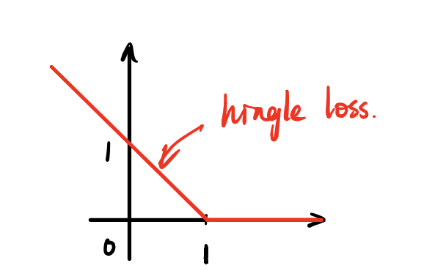
\includegraphics[width=.4\textwidth]{微信图片_20191115131201.png}
    \caption{loss function的展示图}
    \label{fig:my_label_1}
\end{figure}

这个loss function已经是连续的了,而且看起来是不是很像书的开着的样子。所以,它有一个非常形象的名字也就是“合页函数”(Hinge loss)。那么到这里,我们的Soft Margin SVM可以被定义为:
\begin{equation}
    \left\{
        \begin{array}{ll}
        \min \ \frac{1}{2}w^Tw + C\sum_{i=1}^N\max\{ 0, 1-y_i(w^Tx_i+b) \}  & \\
        s.t.\quad y_i(w^Tx_i + b) \geq 1 & \\
    \end{array}
    \right.
\end{equation}

但是,这样写显然不是我们想要的形式,我们需要得到更简便一些的写法。我们引入$\xi_i = 1-y_i(w^Tx_i+b), \ \xi_i \geq 0 $。我们仔细的想一想$\max\{ 0, 1-y_i(w^Tx_i+b) \}$和$\xi_i$之间的关系。有了$\xi_i \geq 0$,我们可以得到其实$\xi_i \geq 0$和$\max\{ 0, 1-y_i(w^Tx_i+b) \}$实际上是等价的。那么这个优化模型我们可以写成:
\begin{equation}
    \left\{
        \begin{array}{ll}
        \min \ \frac{1}{2}w^Tw + C\sum_{i=1}^N\xi_i  & \\
        s.t.\quad y_i(w^Tx_i + b) \geq 1 - \xi_i, \ \xi_i \geq 0 & \\
    \end{array}
    \right.
\end{equation}

在图像上表示即为:
\begin{figure}[H]
    \centering
    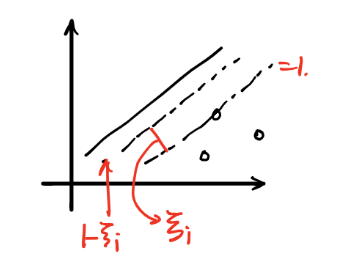
\includegraphics[width=.4\textwidth]{微信图片_20191115134816.png}
    \caption{Soft Margin SVM模型展示图}
    \label{fig:my_label_1}
\end{figure}

在以前的基础上我们增加了一个缓冲区,由于这个缓冲区的存在我们可以允许有点点的误差。而支持向量的区间被放宽到了$1-\xi_i$。

\end{document}
